\documentclass[12pt]{article}

\title{Activity 4: Methods}
\author{Dr. Chris Mayfield}
\date{CS 149, Fall 2016}

%\ProvidesPackage{cspogil}

% fonts
\usepackage[utf8]{inputenc}
\usepackage[T1]{fontenc}
\usepackage{mathpazo}

% spacing
\usepackage[margin=2cm]{geometry}
\renewcommand{\arraystretch}{1.4}
\setlength{\parindent}{0pt}

% orphans and widows
\clubpenalty=10000
\widowpenalty=10000
\pagestyle{empty}

% figures and tables
\usepackage{graphicx}
\usepackage{multicol}
\usepackage{tabularx}
\usepackage{wrapfig}

% fixed-width columns
\usepackage{array}
\newcolumntype{L}[1]{>{\raggedright\let\newline\\\arraybackslash\hspace{0pt}}m{#1}}
\newcolumntype{C}[1]{>{\centering\let\newline\\\arraybackslash\hspace{0pt}}m{#1}}
\newcolumntype{R}[1]{>{\raggedleft\let\newline\\\arraybackslash\hspace{0pt}}m{#1}}

% include paths
\makeatletter
\def\input@path{{Models/}{../../Models/}}
\graphicspath{{Models/}{../../Models/}}
\makeatother

% colors
\usepackage[svgnames,table]{xcolor}
\definecolor{bgcolor}{HTML}{FAFAFA}
\definecolor{comment}{HTML}{007C00}
\definecolor{keyword}{HTML}{0000FF}
\definecolor{strings}{HTML}{B20000}

% table headers
\newcommand{\tr}{\bf\cellcolor{Yellow!10}}

% syntax highlighting
\usepackage{textcomp}
\usepackage{listings}
\lstset{
    basicstyle=\ttfamily\color{black},
    backgroundcolor=\color{bgcolor},
    numberstyle=\scriptsize\color{comment},
    commentstyle=\color{comment},
    keywordstyle=\color{keyword},
    stringstyle=\color{strings},
    columns=fullflexible,
    keepspaces=true,
    showlines=true,
    showstringspaces=false,
    upquote=true
}

% code environments
\newcommand{\java}[1]{\lstinline[language=java]{#1}}%[
\lstnewenvironment{javalst}{\lstset{language=java,backgroundcolor=}}{}
\lstnewenvironment{javabox}{\lstset{language=java,frame=single,numbers=left}\quote}{\endquote}

% PDF properties
\usepackage[pdftex]{hyperref}
\urlstyle{same}
\makeatletter
\hypersetup{
  pdftitle={\@title},
  pdfauthor={\@author},
  pdfsubject={\@date},
  pdfkeywords={},
  bookmarksopen=false,
  colorlinks=true,
  citecolor=black,
  filecolor=black,
  linkcolor=black,
  urlcolor=blue
}
\makeatother

% titles
\makeatletter
\renewcommand{\maketitle}{\begin{center}\LARGE\@title\end{center}}
\makeatother

% boxes [optional height]
\newcommand{\emptybox}[1][10em]{
\vspace{1em}
\begin{tabularx}{\linewidth}{|X|}
\hline\\[#1]\hline
\end{tabularx}}

% models
\newcommand{\model}[1]{\section{#1}\nopagebreak}
\renewcommand{\thesection}{Model~\arabic{section}}

% questions
\newcommand{\quest}[1]{\subsection*{Questions~ (#1)}}
\newcounter{question}
\newcommand{\Q}{\vspace{1em}\refstepcounter{question}\arabic{question}.~ }
\renewcommand{\thequestion}{\#\arabic{question}}

% sub-question lists
\usepackage{enumitem}
\setenumerate[1]{label=\alph*)}
\setlist{itemsep=1em,after=\vspace{1ex}}

% inline answers
\definecolor{answers}{HTML}{C0C0C0}
\newcommand{\ans}[1]{%
\ifdefined\Student
    \leavevmode\phantom{~~\textcolor{answers}{#1}}
\else
    ~~\textcolor{answers}{#1}
\fi}

% longer answers [optional height]
\newsavebox{\ansbox}
\newenvironment{answer}[1][4em]{
\nopagebreak
\begin{lrbox}{\ansbox}
\begin{minipage}[t][#1]{\linewidth}
\color{answers}
}{
\end{minipage}
\end{lrbox}
\ifdefined\Student
    \phantom{\usebox{\ansbox}}%
\else
    \usebox{\ansbox}%
\fi}


\begin{document}

\maketitle

Java programs are organized into {\em classes}, each of which has one or more {\em methods}, each of which has one or more {\em statements}.
Writing methods allows you to break down a complex program into smaller blocks of reusable code.

\model{Invoke and Return}

Each statement in this program \emph{invokes} (or calls) a method.
At the end of a method, Java \emph{returns} to where it was invoked.
The list of events on the right illustrates how the program runs.

\vspace{3ex}

\begin{minipage}{0.68\textwidth}
\begin{javabox}
public class Model {
    
    public static void main(String[] args) {
        System.out.println("First line.");
        threeLine();
        System.out.println("Second line.");
    }
    
    public static void newLine() {
        System.out.println();
    }
    
    public static void threeLine() {
        newLine();
        newLine();
        newLine();
    }
    
}
\end{javabox}
\end{minipage}
\hfill
\begin{minipage}{0.34\textwidth}
\begin{verbatim}

INVOKE println
RETURN to line 5
INVOKE threeLine
    INVOKE newLine
        INVOKE println
        RETURN to line 11
    RETURN to line 15
    INVOKE newLine
        INVOKE println
        RETURN to line 11
    RETURN to line 16
    INVOKE newLine
        INVOKE println
        RETURN to line 11
    RETURN to line 17
RETURN to line 6
INVOKE println
RETURN to line 7

\end{verbatim}
\end{minipage}


\quest{15 min}


\Q \label{lines}
How many lines of source code invoke the \java{println} method? \ans[10em]{Three (lines 4, 6, 10)}
\vspace{1em}


\Q \label{times}
How many times is \java{println} invoked when the program runs? \ans[10em]{Five times}
\vspace{1em}


\Q For each \texttt{INVOKE} on the right, draw an arrow to the corresponding line of code.
(Plan ahead so that crossing lines will still be legible.) %\ans{There should be 9 lines total.}
\vspace{1em}


\Q What is the output of the program? Please write \java{\\n} to show each newline character.

\begin{answer}[8em]
\vspace{-1ex}
\begin{javaans}
First line.\n
\n
\n
\n
Second line.\n
\end{javaans}
\end{answer}


\Q When Java sees a name like \java{x}, \java{count}, or \java{newLine}, how can it tell whether it's a variable or a method? (Hint: syntax)

\begin{answer}[5em]
Methods have parentheses, and variables do not.
They are similar to functions in math  : when you see $g(x)$, you know that $g$ is a function and $x$ is a variable.
\end{answer}


\Q What is the difference between a method and a variable? What do they have in common?

\begin{answer}[5em]
All computer programs, regardless of language, consist of \emph{code} and \emph{data}.
Methods contain code (statements or instructions), whereas variables contain data (references or values).
\end{answer}


\Q In your own words, describe what methods are for. Why not just write everything in \java{main}?

\begin{answer}[5em]
Methods help organize the code into separate parts.
They also make it possible to write code once and use it multiple times.
\end{answer}

%\newpage
\model{Math Methods}

Consider the following methods defined in the \java{Math} class:

\begin{javalst}
    public static int abs(int a)
    public static double log(double a)
    public static double pow(double a, double b)
    public static double random()
    public static int subtractExact(int x, int y)
\end{javalst}

Note this list isn't exhaustive; \java{Math} has over 70 methods in total.
To invoke methods from another class (like \java{Math}), you must first specify the class name:

\begin{javalst}
    value = abs(-5);       // Error: cannot find symbol
    value = Math.abs(-5);  // correct
\end{javalst}

The period in this example is called the \emph{dot operator}. When reading the above code out loud, you would say ``math dot abs''.

Here is the Java documentation for the methods listed above:
\nopagebreak
\begin{center}
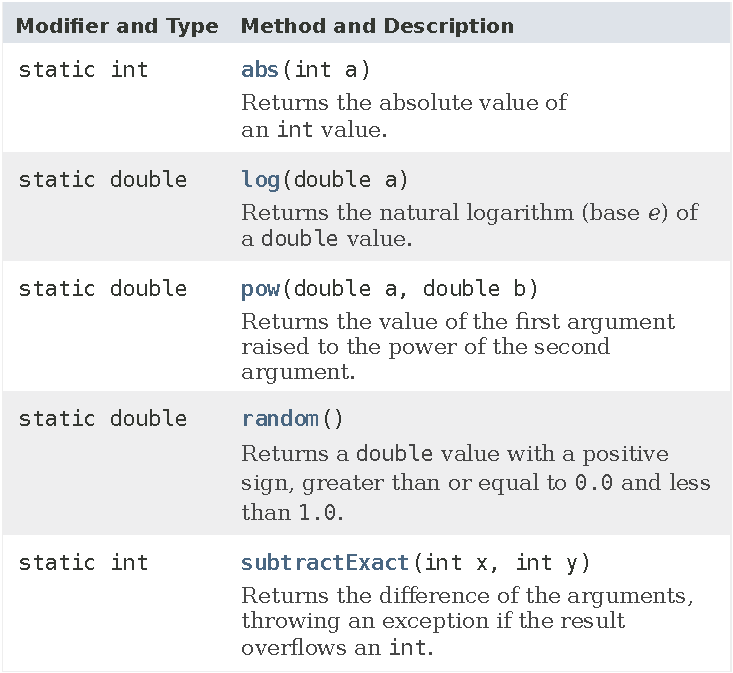
\includegraphics[scale=0.90]{math-javadoc.pdf}
\end{center}


\quest{15 min}


\Q What type of value does \java{Math.random()} return? Give an example of what it would look like.

\begin{answer}
It returns a random \texttt{double} value greater than or equal to 0.0 and less than 1.0.
For example, the value 0.7851637186510342.
\end{answer}


\Q When \emph{invoking} a method, what do you need to specify before and after the method name?

\begin{answer}
Before the name, you need to specify the class name (unless the method is in the same class).
After the name, you need to specify the required values.
\end{answer}


\Q For each method, write a Java statement that invokes it and assigns the result to a variable.

\begin{answer}[8em]
\vspace{-1ex}
\begin{javaans}
answer = Math.abs(-5);
length = Math.log(1.2);
amount = Math.pow(3.4, 5.6);
number = Math.random();
result = Math.subtractExact(-78, 90);
\end{javaans}
\end{answer}


\Q When \emph{defining} a method, what do you need to specify before and after the method name?

\begin{answer}
Before the name, you need to specify what type of value the method will return.
After the name, you need to specify what values are required to invoke the method.
\end{answer}


\Q Define a method named \java{average} that requires two integers \java{x} and \java{y} and returns a \java{double}. (Don't write any semicolons or braces.)

\begin{answer}
\begin{javaans}
public static double average(int x, int y)
\end{javaans}
\end{answer}


\comment{
What you wrote for the previous question is called the method's \textbf{signature}.
The variables declared inside the parentheses are called \textbf{parameters}.
When invoking the method, the values you provide are called \textbf{arguments}.
Since arguments will be assigned to parameters, their types must be compatible.
}


\Q How many parameters and arguments does each method have?

\begin{center}
\begin{tabular}{|c|C{1in}|C{1in}|}
\hline
\tr Method & \tr \# Params & \tr \# Args \\
\hline
\java{abs} & \ans{1} & \ans{1} \\
\hline
\java{log} & \ans{1} & \ans{1} \\
\hline
\java{pow} & \ans{2} & \ans{2} \\
\hline
\java{random} & \ans{0} & \ans{0} \\
\hline
\java{subtractExact} & \ans{2} & \ans{2} \\
\hline
\java{println} & \ans{1} & \ans{1} \\
\hline
\end{tabular}
\end{center}


\Q Consider the statement \java{System.out.println("Price: " + price);} where the value of \java{price} is 9.99. What is the argument that \texttt{println} receives?

\begin{answer}
\begin{javaans}
"Price: 9.99"
\end{javaans}
\end{answer}


\Q Consider the statement \java{System.out.printf("Price: \%f", price);} where the value of \java{price} is 9.99. Why does \java{println} use \emph{plus} and \java{printf} use \emph{comma} to specify the arguments?

\begin{answer}[5em]
The \java{println} method requires only one argument, so plus in this context means concatenate.
The \java{printf} method requires multiple arguments: one for the format string, and others for the values to substitute.
\end{answer}

\model{Stack Diagrams}

Each method has its own area of memory to store parameters and other variables.
When a method is invoked, Java allocates this memory on the \emph{call stack}.
For convenience, we draw ``stack'' diagrams upside down.

\begin{center}
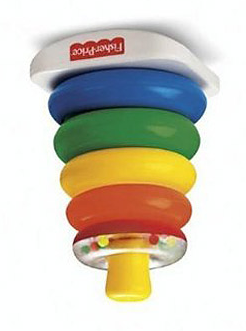
\includegraphics[height=3in]{stack-rings1.png}
\hspace{1em}
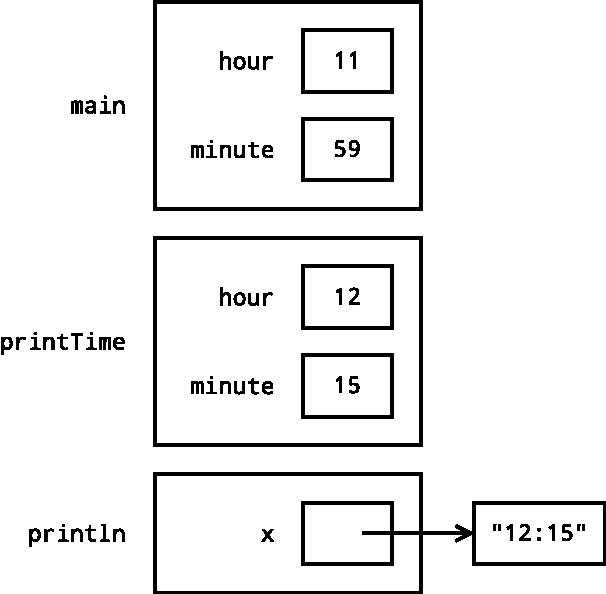
\includegraphics[height=3in]{stack1.pdf}
\end{center}

\begin{center}
Note: The signature for \java{System.out.println} is ~\java{public void println(String x)}.
\end{center}

\begin{javalst}
    public static void printTime(int hour, int minute) {
        System.out.println(hour + ":" + minute);
    }
    
    public static void main(String[] args) {
        int hour = 11;
        int minute = 59;
        printTime(12, 15);
    }
\end{javalst}


\quest{15 min}


\Q Based on the diagram, how many methods does the program call? \ans{Three}
\vspace{1ex}


\Q Based on the diagram, how many variables does the program have? \ans{Five}
\vspace{1ex}


\Q How do stack diagrams extend the memory diagrams we've seen previously?

\begin{answer}[5em]
There is a box for each method call, with the name of the method on the left.
Note that reference types (like strings) are not stored ``on the stack'' --- the variables are part of the method, but the actual data is outside of the method.
\end{answer}


\Q How is it possible that two variables with the same name can have different values?

\begin{answer}
Each method declares its own variables.
Because they are stored in different memory locations, the values are independent from other methods.
\end{answer}


\Q \label{drawing}
Draw a stack diagram to show the state of memory just before \java{println} is called.
Assume the user inputs the value 10.
(You should be able to do this kind of math without a calculator.)

\vspace{1ex}
\begin{javalst}
    public static void show(double c) {
        double f;
        String str;
        f = c * 1.8 + 32;
        str = String.format("%.1f C = %.1f F\n", c, f);
        System.out.println(str);
    }

    public static void main(String[] args) {
        double c;
        Scanner in = new Scanner(System.in);
        System.out.print("Enter temperature in Celsius: ");
        c = in.nextDouble();
        show(c);
    }
\end{javalst}
\vspace{-1ex}

\begin{answer}[3.1in]
\hfill
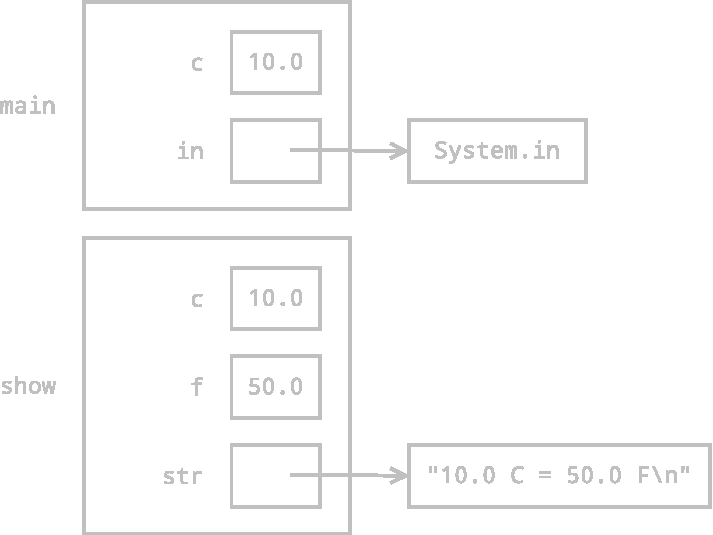
\includegraphics[height=3in]{stack2.pdf}
\end{answer}


\Q What is the difference between the \java{String.format} method (used in the previous question) and \java{System.out.printf}?

\begin{answer}
They both substitute values based on format specifiers.
\java{String.format} returns a new string, whereas \java{System.out.printf} displays it on the screen.
(In fact, \java{System.out.printf} invokes the \java{String.format} method.)
\end{answer}


\end{document}
